Kate Starbird of University of Washington
\href{https://web.archive.org/web/20221104213000/https://twitter.com/katestarbird/status/1588589381266599936}{said
something important on Twitter earlier today}:

\begin{figure}
\centering
\pandocbounded{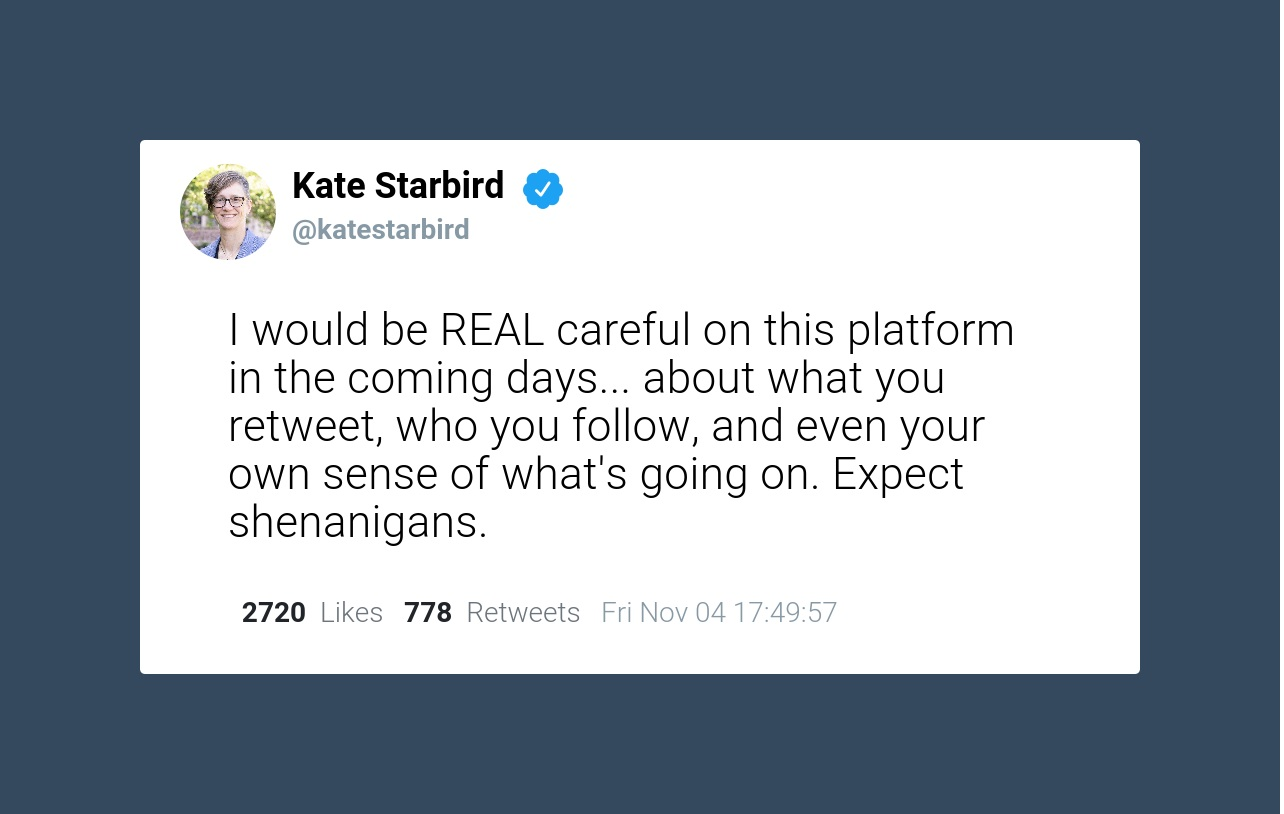
\includegraphics[keepaspectratio]{\%7B\%7Bsite.url\%7D\%7D/img/careful-on-fail-whale.jpeg}}
\caption{Screen capture of tweet by Kate Starbird}
\end{figure}

\emph{Original URL was
\url{https://twitter.com/katestarbird/status/1588589381266599936}}

Twitter has been having issues today since the layoffs took place at
1600 UTC. The entire Accessibility team is gone as is the Curation team
reportedly. Apparently the Human Rights team is gone too if reports are
to be believed.

The guys at \href{https://rifftrax.com/}{RiffTrax} are starting to
abandon ship on Twitter as they're pointing people to Instagram and
Tumblr. While not surprising it is still sad. Bill Corbett is walking
away from his Twitter account and I'm not sure what Kevin and Mike are
doing.

This blog will likely be the way forward as Twitter's implosion
continues. I'm not looking at jumping to Mastodon. That realm is just
too frakking weird. As long as it is up
\href{https://identi.ca/alpacaherder}{my account on Identica still
exists} after all these years even in the \texttt{pump.io} era. I may
look at
\href{https://en.wikipedia.org/w/index.php?title=Secure_Scuttlebutt&oldid=1116253870}{Secure
Scuttlebutt} potentially once I get through my current work tasking.

Life is full of change but you don't expect to hit you so fast and so
bunched up.
